\section{Exploratory Data Analysis}
The three sets of data explained in the last section were composed of one large, accelerometer dataset that contained data points for all the participants.
And the remaining two were a raw and clean version of the TAC data per participant.
In order to extract more features we had to merge the three sets into one complete dataset.
The data needed some preprocessing, before feature extraction, which is the purpose of this section.
The accelerometer sets (Figure \ref{fig:acc-comp}) for one, sampled at $40 \si{\hertz}$ contained many more points as opposed to the data from the bracelets (Figure \ref{fig:tac-comp}), captured once every $30$ minutes.
Another problem was that the accelerometer data often contained gaps for various reasons including phone power outages.
\begin{figure}[h]
	\begin{subfigure}[c]{0.49\columnwidth}
		\centering
		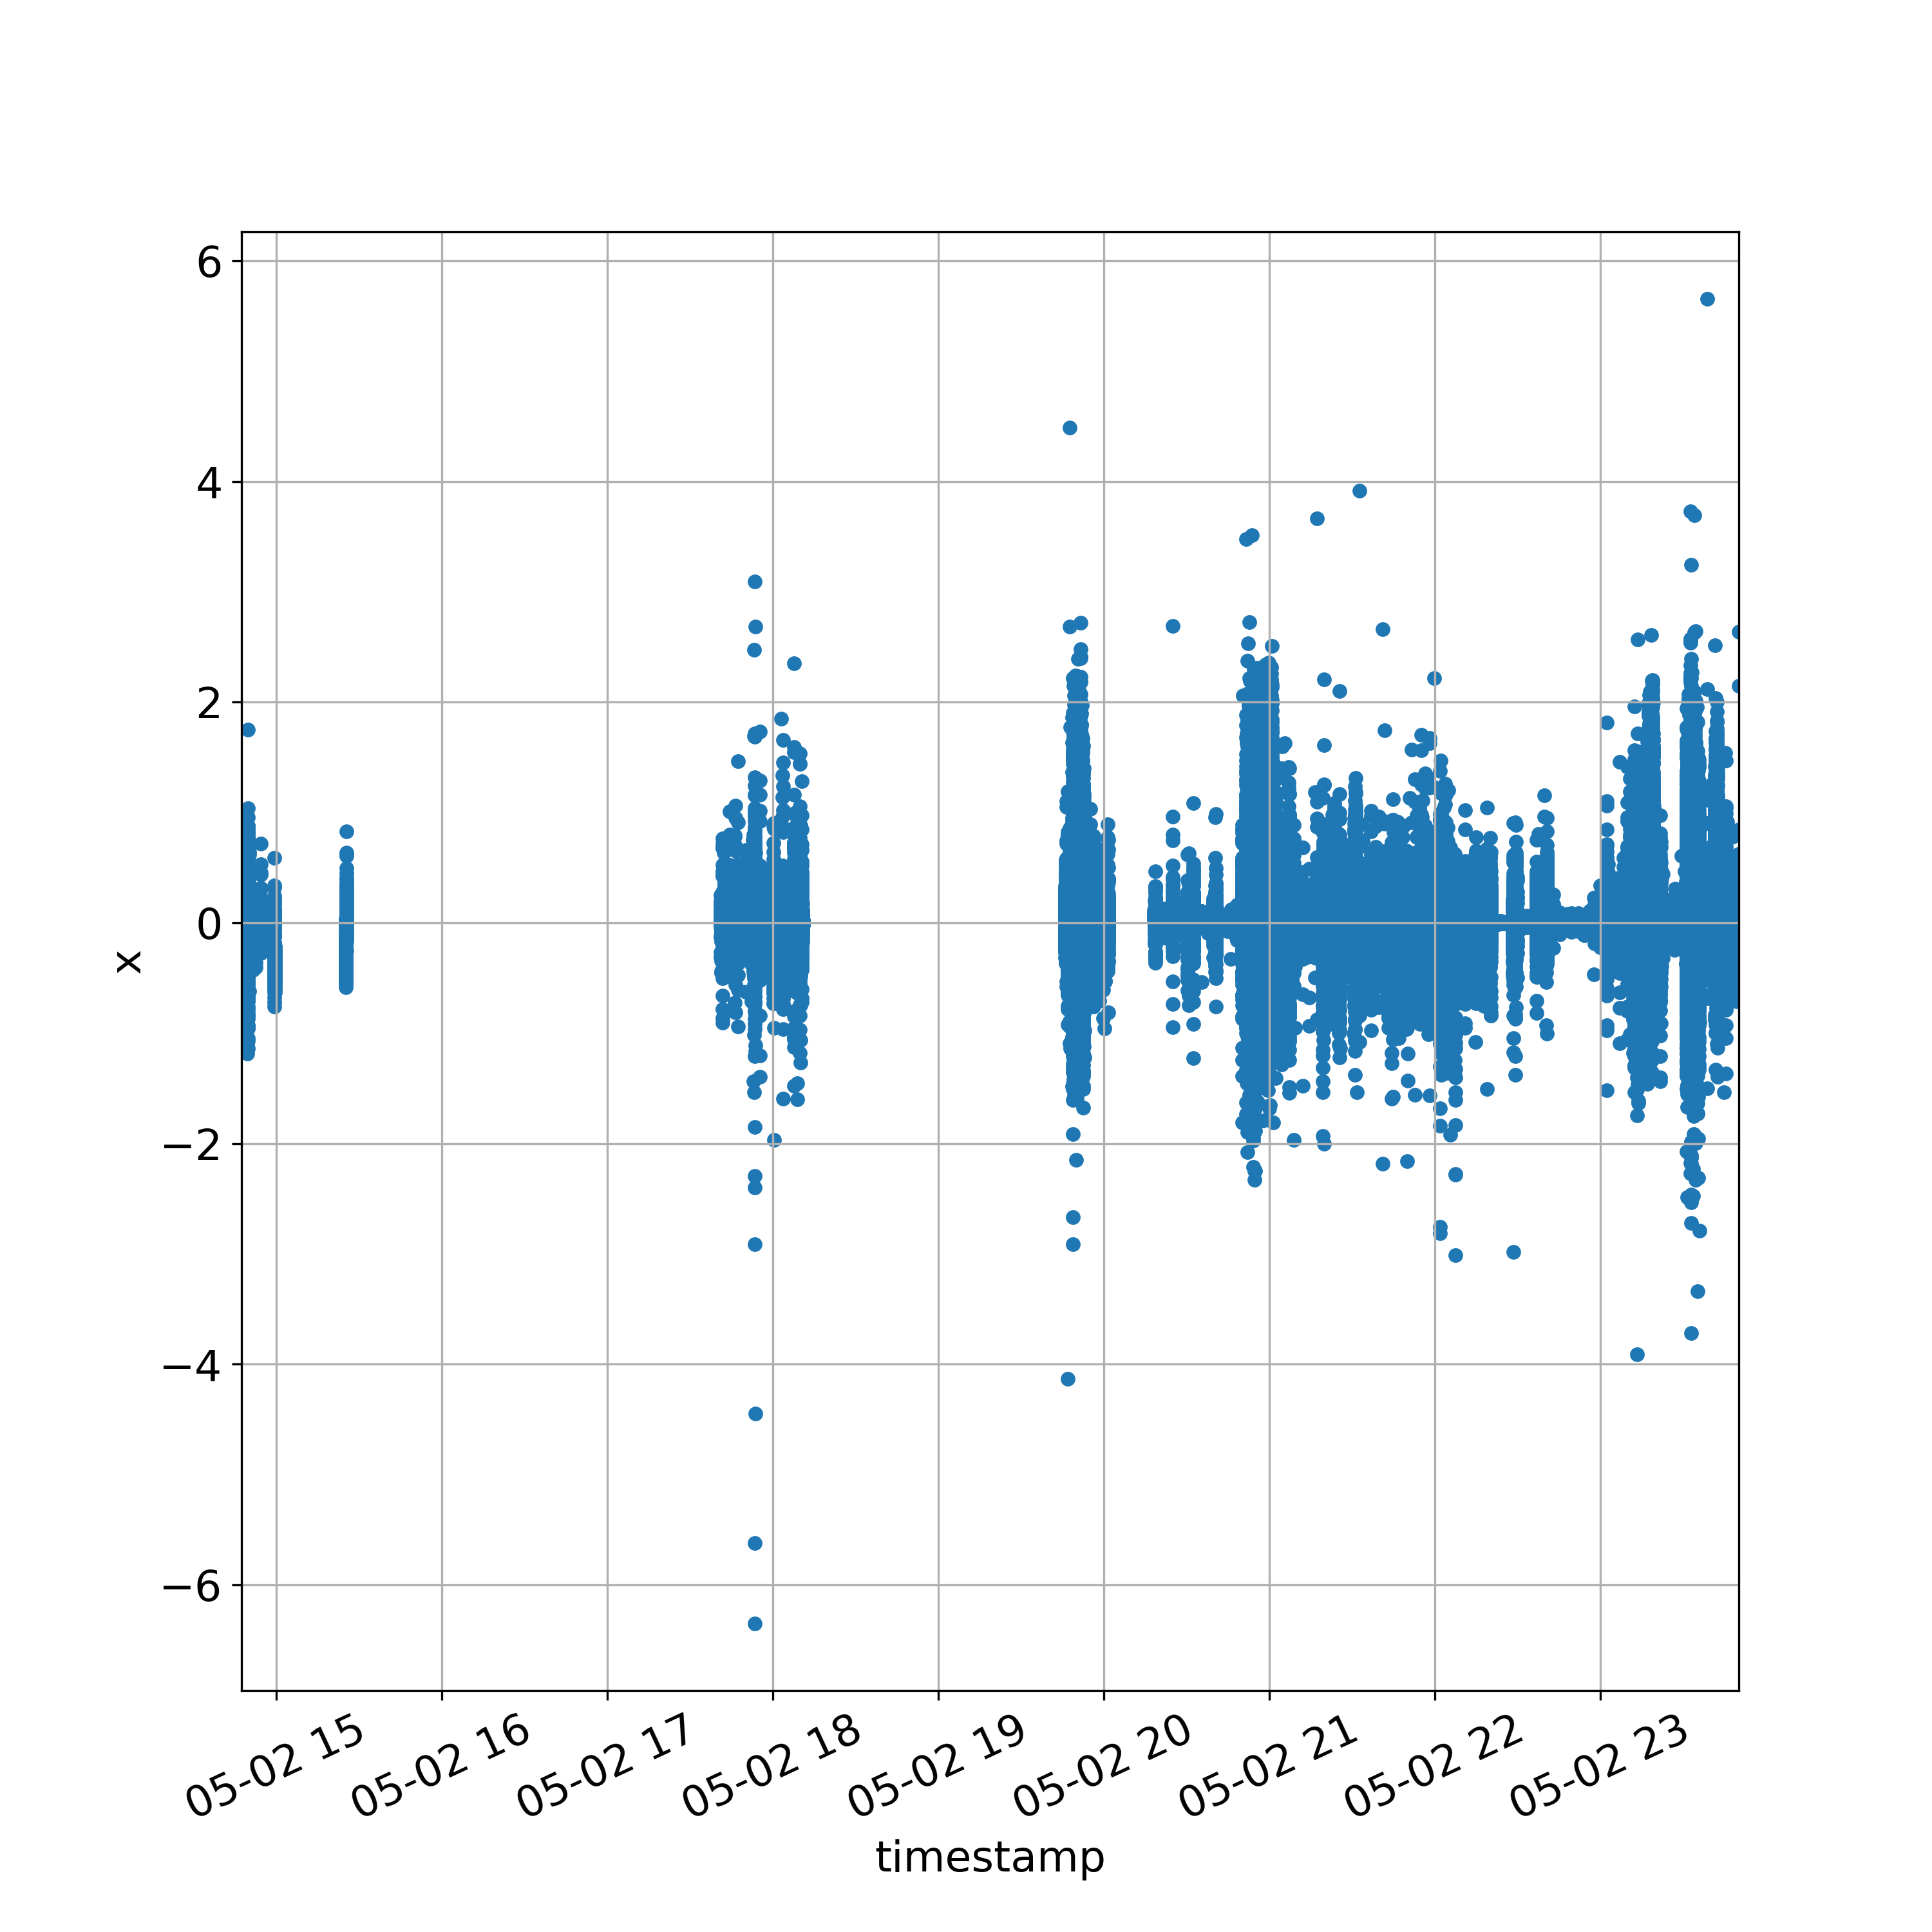
\includegraphics[width=\textwidth]{DC6359_acc_x}
		\caption{Original}
		\label{fig:acc-orig}		
	\end{subfigure}\hfill%
	\begin{subfigure}[c]{0.49\columnwidth}
		\centering
		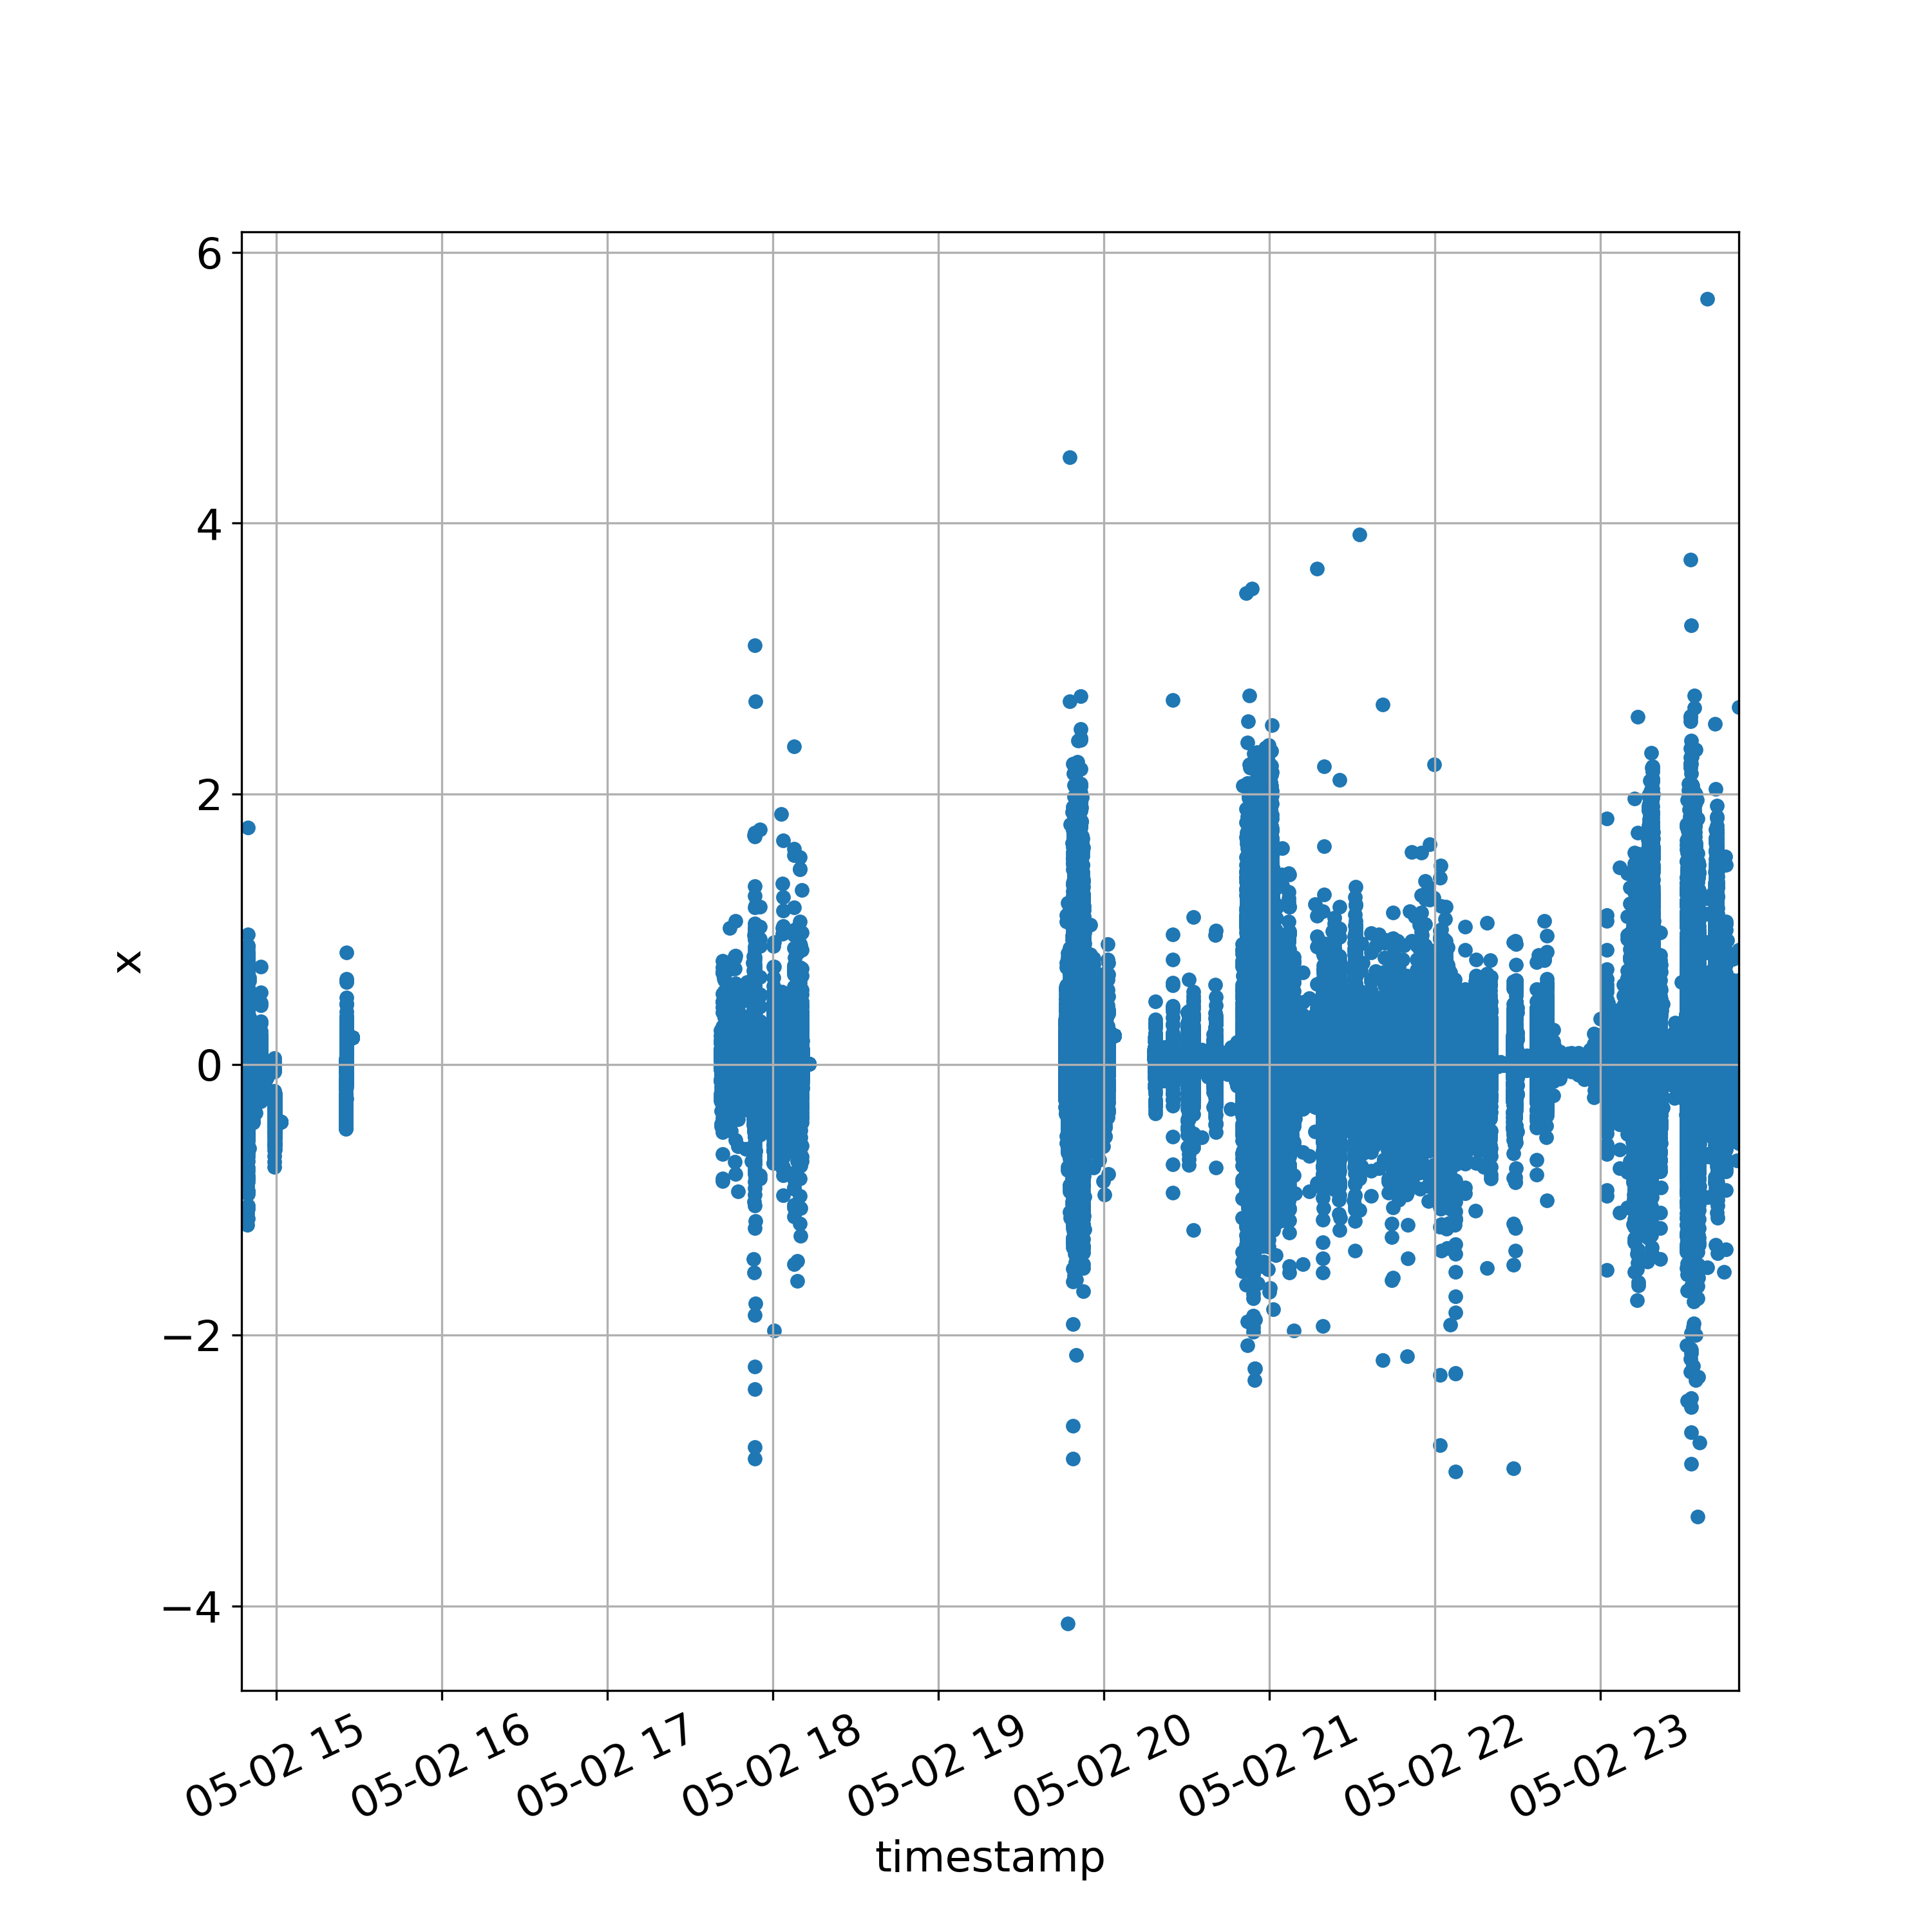
\includegraphics[width=\textwidth]{DC6359_merged_x}
		\caption{Resampled and interpolated}
		\label{fig:acc-intpl}
	\end{subfigure}
	\caption{Comparison of accelerometer data for sample \texttt{DC6359}}
	\label{fig:acc-comp}
\end{figure}
\begin{figure}[h]
	\begin{subfigure}[c]{0.49\columnwidth}
		\centering
		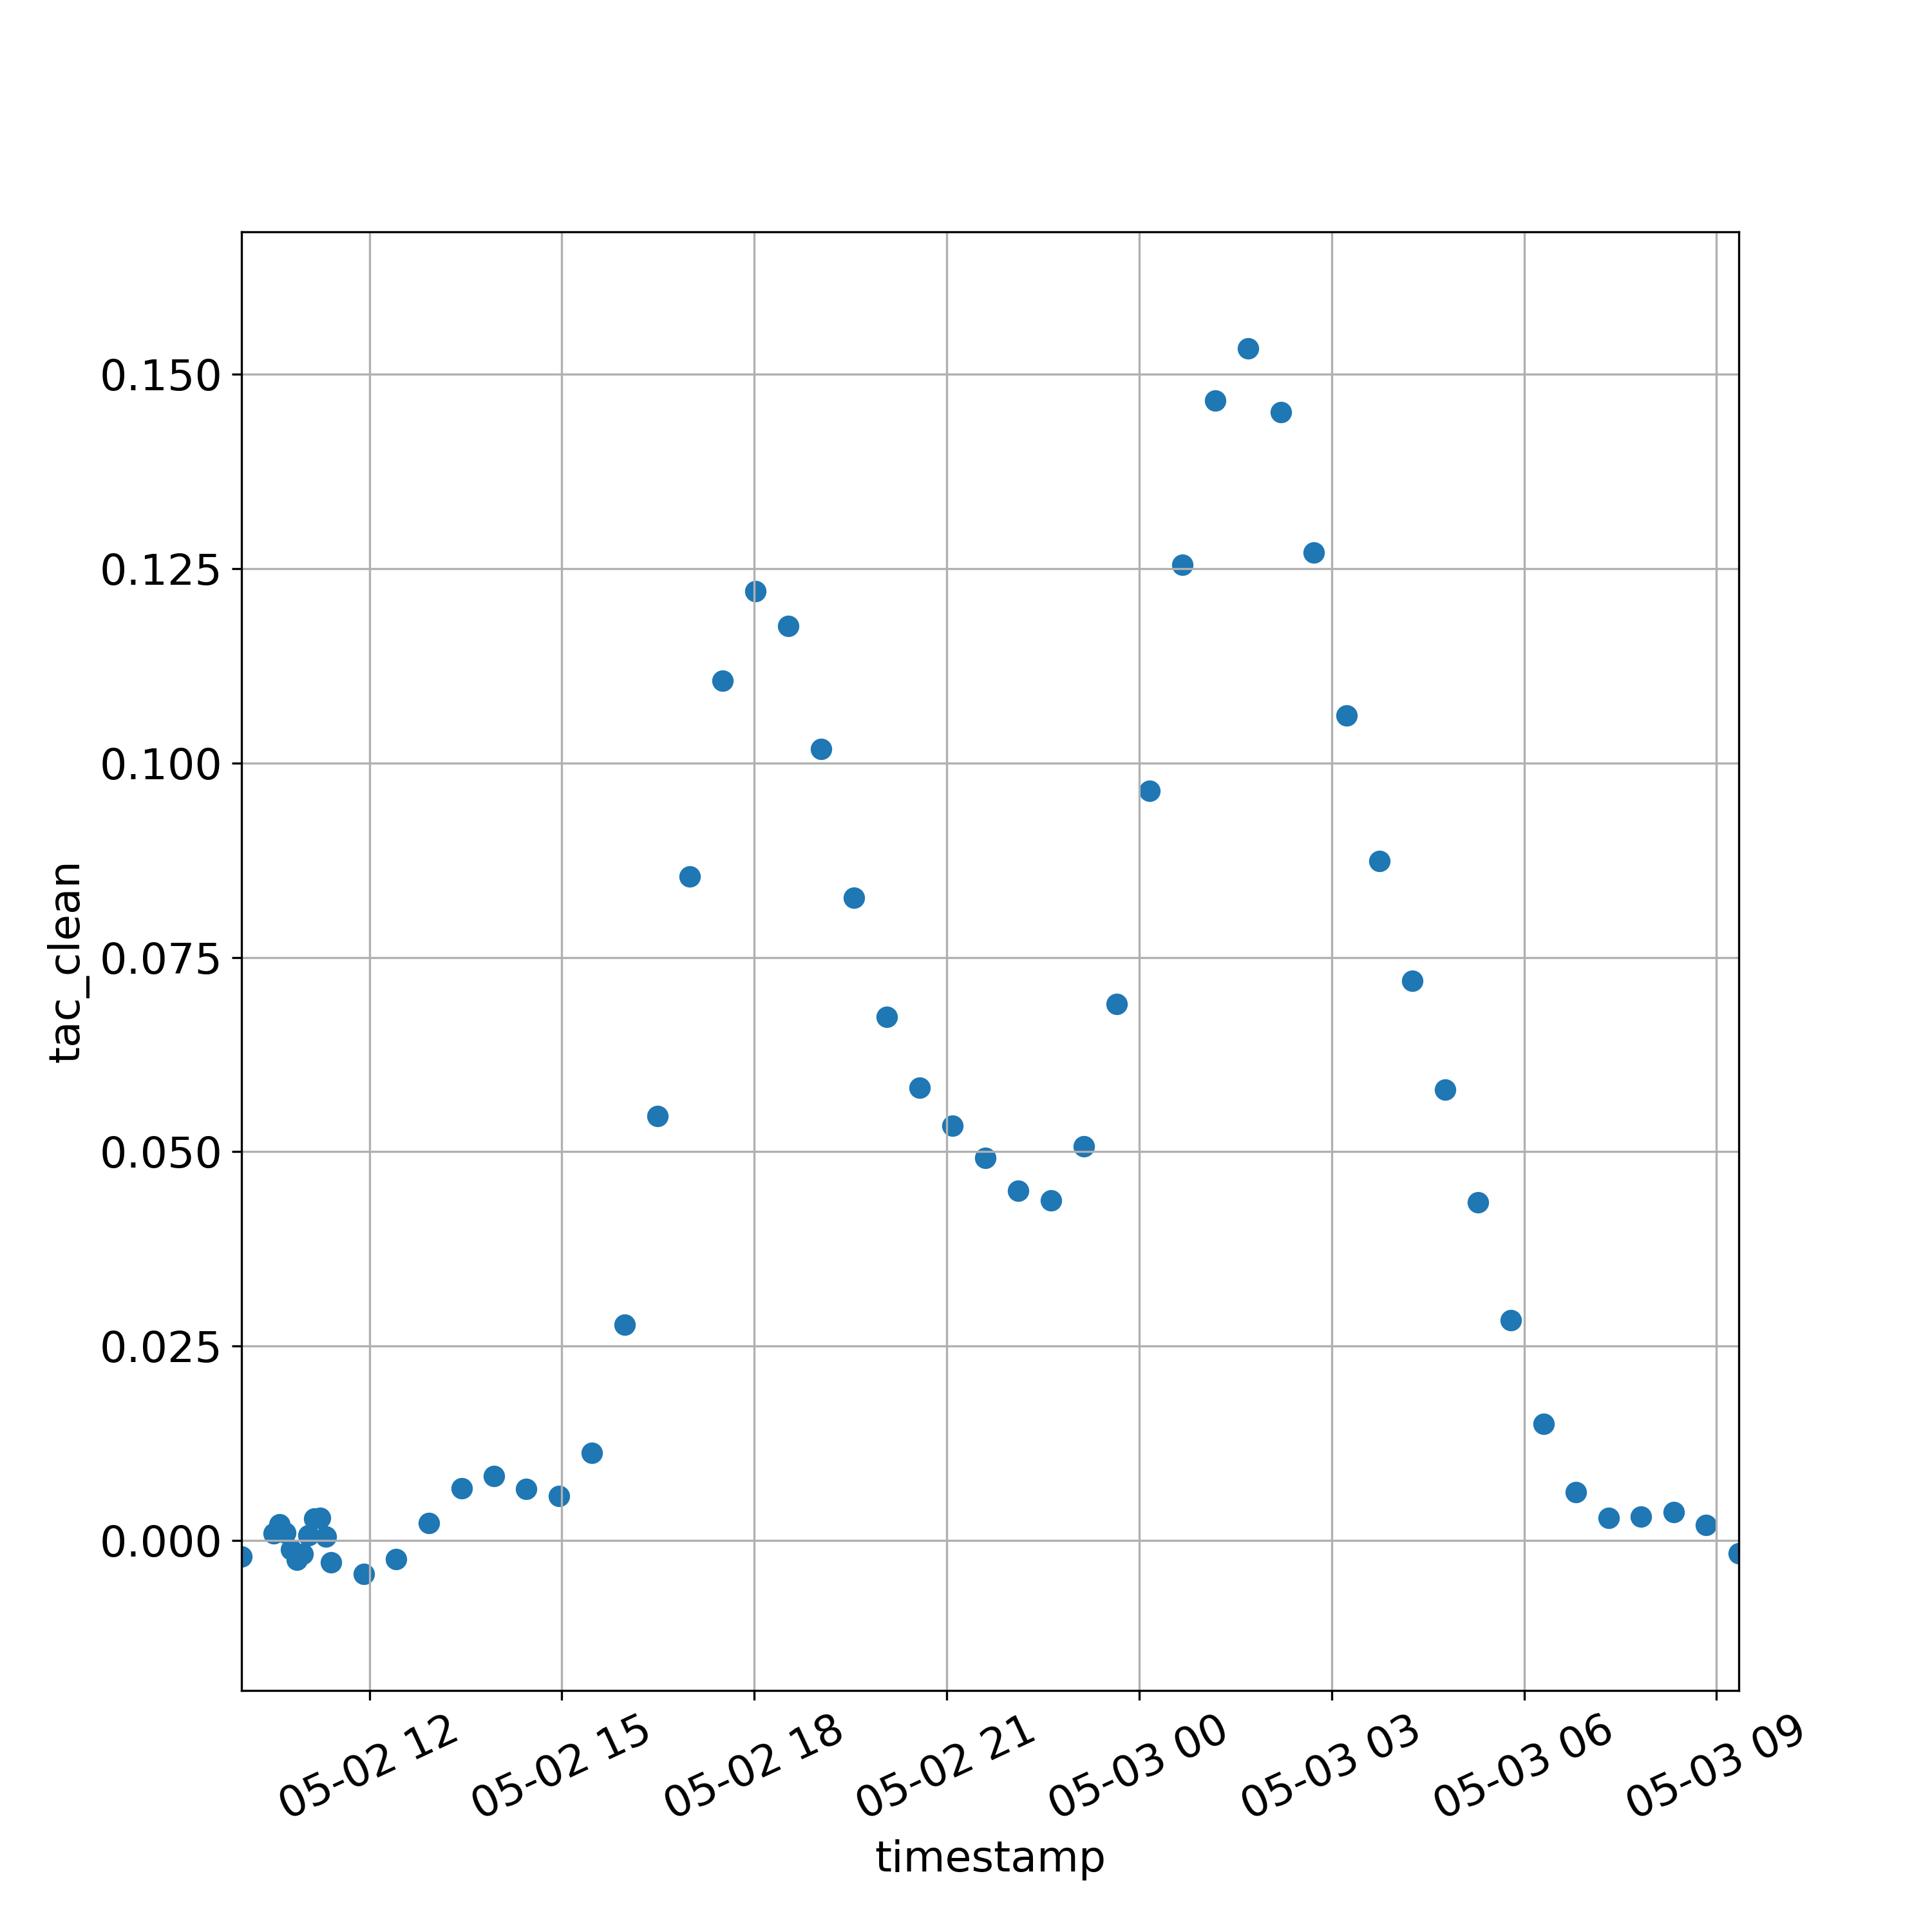
\includegraphics[width=\textwidth]{DC6359_tac_clean}
		\caption{Original}
		\label{fig:tac-orig}		
	\end{subfigure}\hfill%
	\begin{subfigure}[c]{0.49\columnwidth}
		\centering
		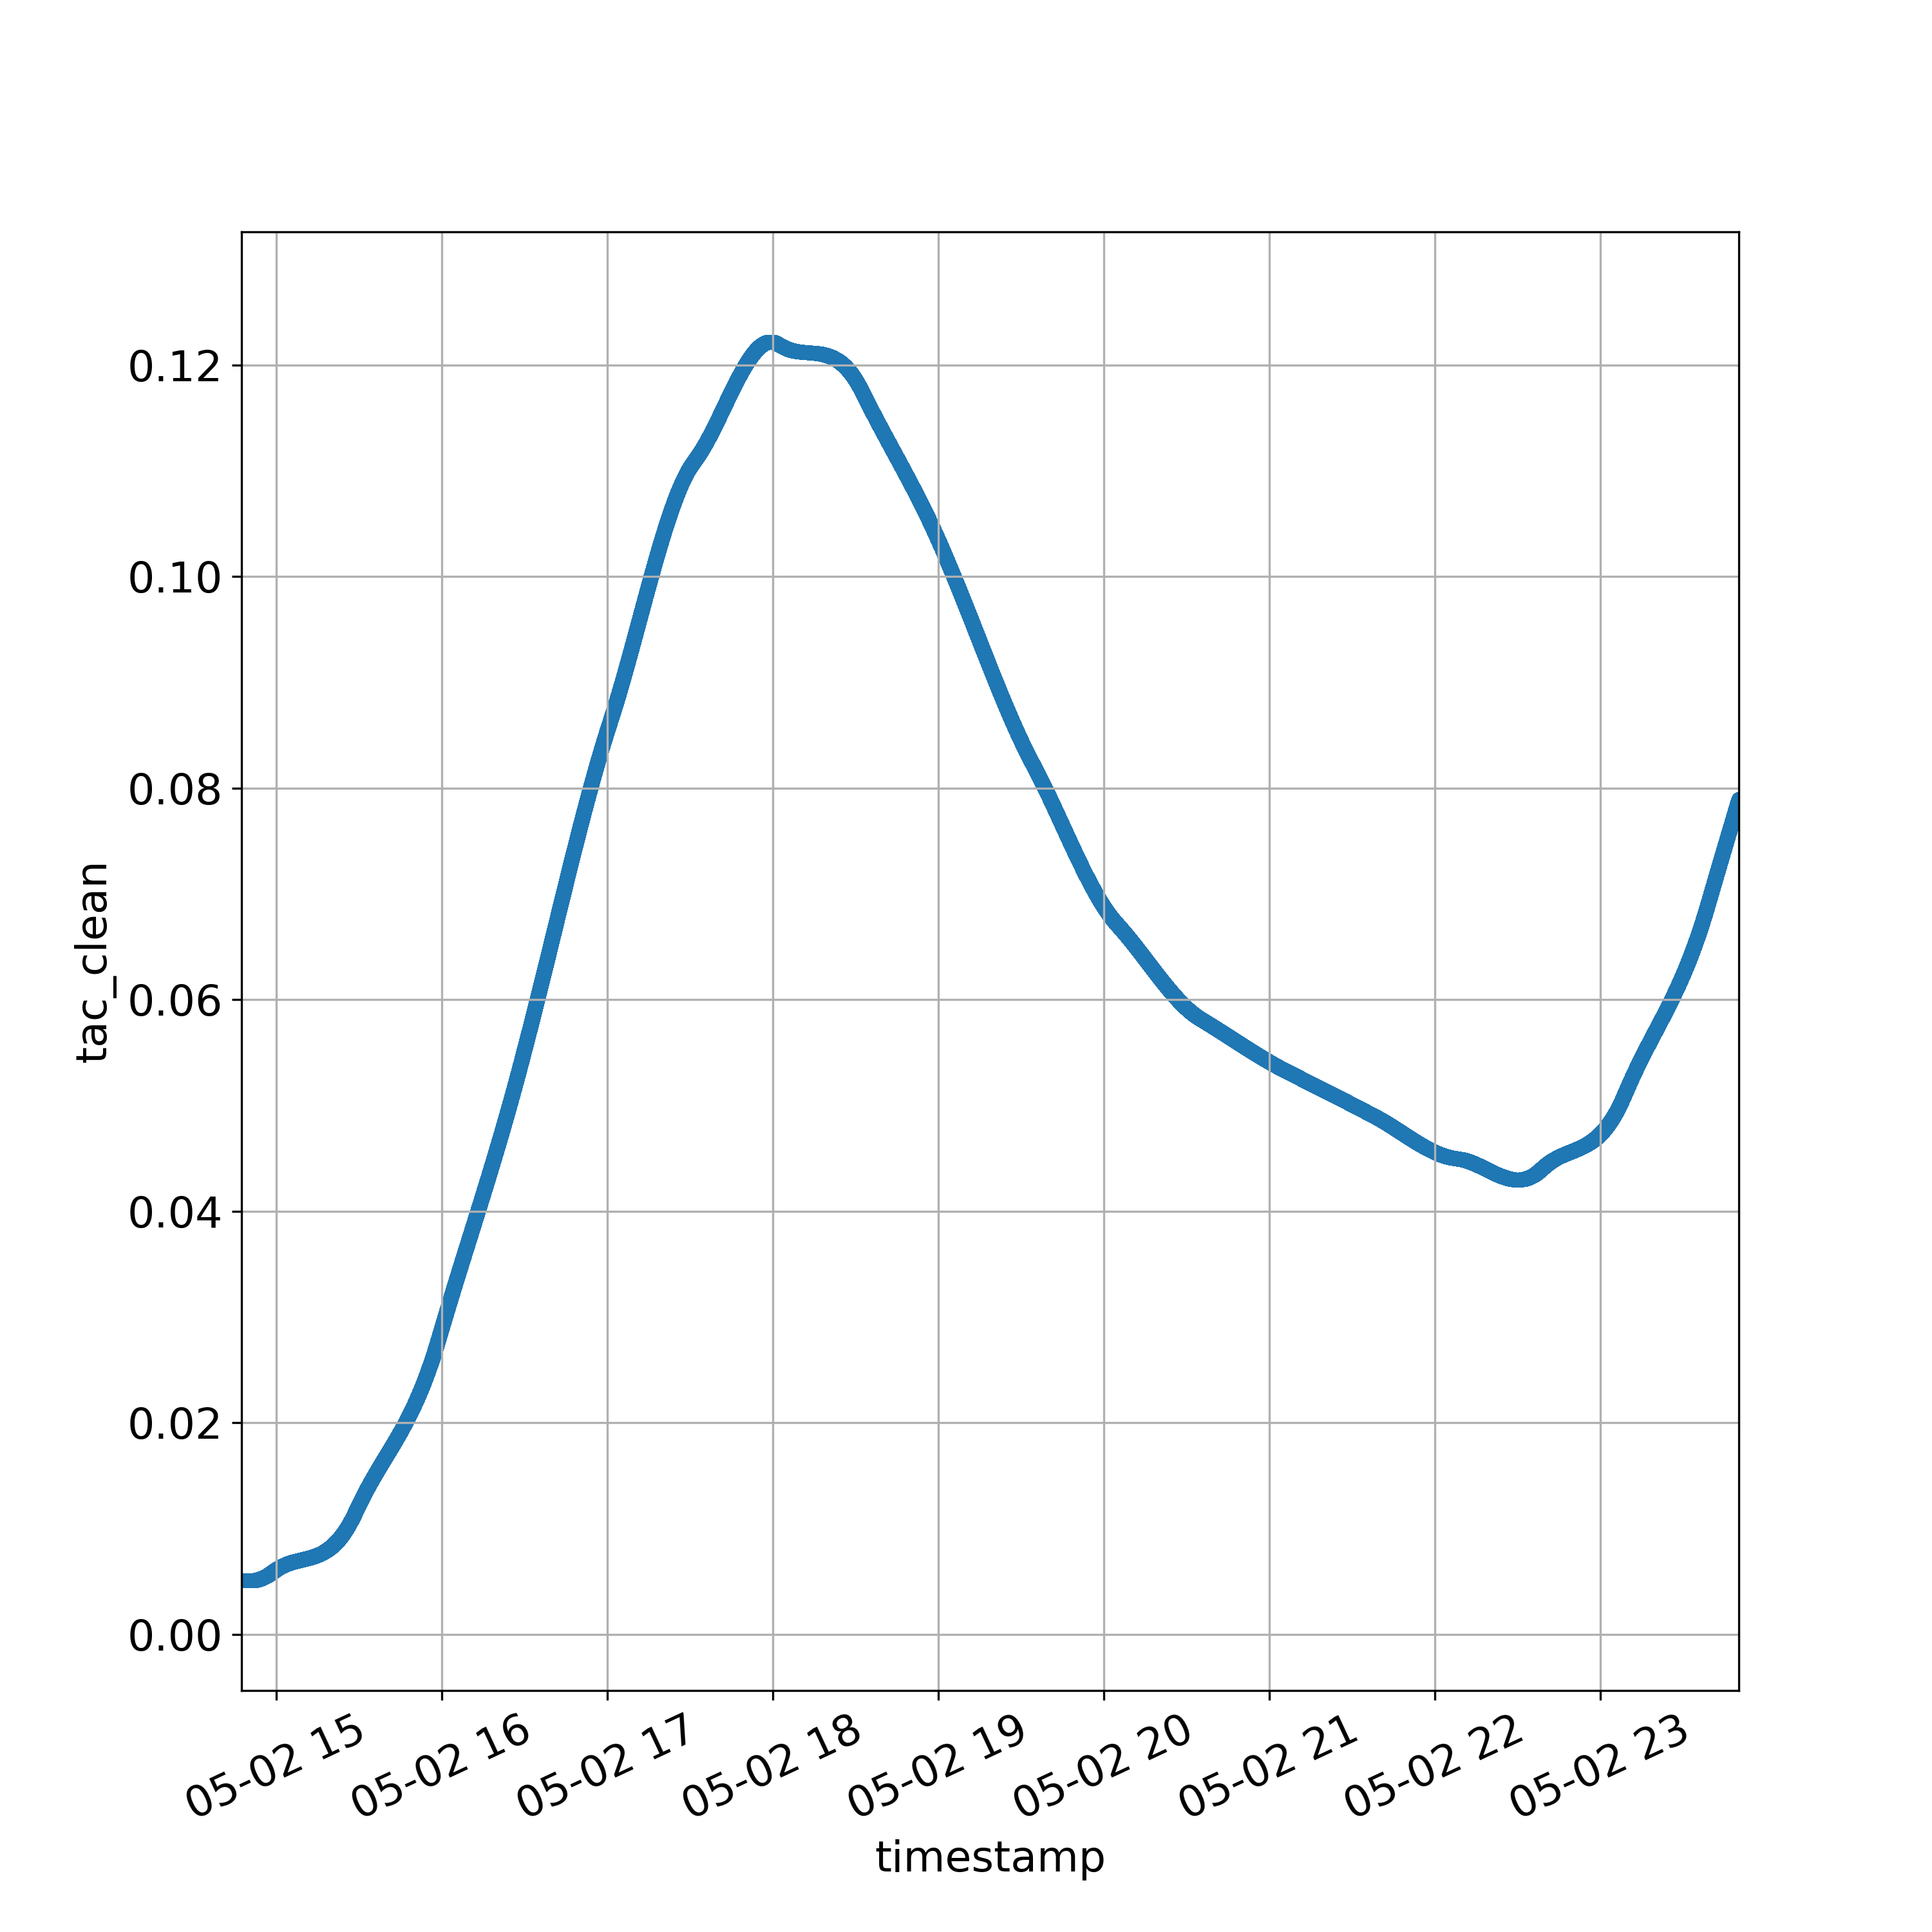
\includegraphics[width=\textwidth]{DC6359_merged_clean}
		\caption{Cropped, resampled and interpolated}
		\label{fig:tac-intpl}
	\end{subfigure}
	\caption{Comparison of TAC data for sample \texttt{DC6359}}
	\label{fig:tac-comp}
\end{figure}
We splitted accelerometer data to contain points for each user independently and then merged raw and clean TAC datasets together to have both attributes into one set before a final combination of all three.
In order to prevent target leakage and the raw readings were later dropped again.
Even though the dataset is apparently recorded at $40\si{\hertz}$, the merged set did not contain equally spaced timestamps, so we resampled the data at $25\si{\milli\second}$ to get an equally distanced time series.
We then interpolated the data linearly to makeup for the missing TAC points lying in between the frequently sampled accelerometer points.
There was a threshold however in order to not interpolate over the large areas, missing accelerometer data points, so we could cut them out later.
The results are visible in a few extra data points on the end of each gap in Figure \ref{fig:acc-intpl} showing merged accelerometer data before hitting the threshold.
Apart from these points the data is very similar.
Another interpolation was applied to the TAC data exclusively employing the 'akima spline' method.
This is visualized in the two plots shown in Figure \ref{fig:tac-comp}.
Notice that both are scatter plots, but the second one consists of much denser data points.
Also, the second plot consists only of the first and the last valid accelerometer data timestamps.
Finally we removed the missing gaps in between the data points by splitting the time series into chunks where only a valid combination of both, accelerometer and TAC data were present.
A chunk of the same dataset is visible in Figure \ref{fig:acc-chunk} depicting the fifth chunk of the accelerometer data and in Figure \ref{fig:tac-chunk} the TAC clean data points of the same gap between 20:00 and 12:00.
The process was repeated for each chunk of valid data until valid sets of clean, continuous data was achieved.

\begin{figure}[h]
	\begin{subfigure}[c]{0.49\columnwidth}
		\centering
		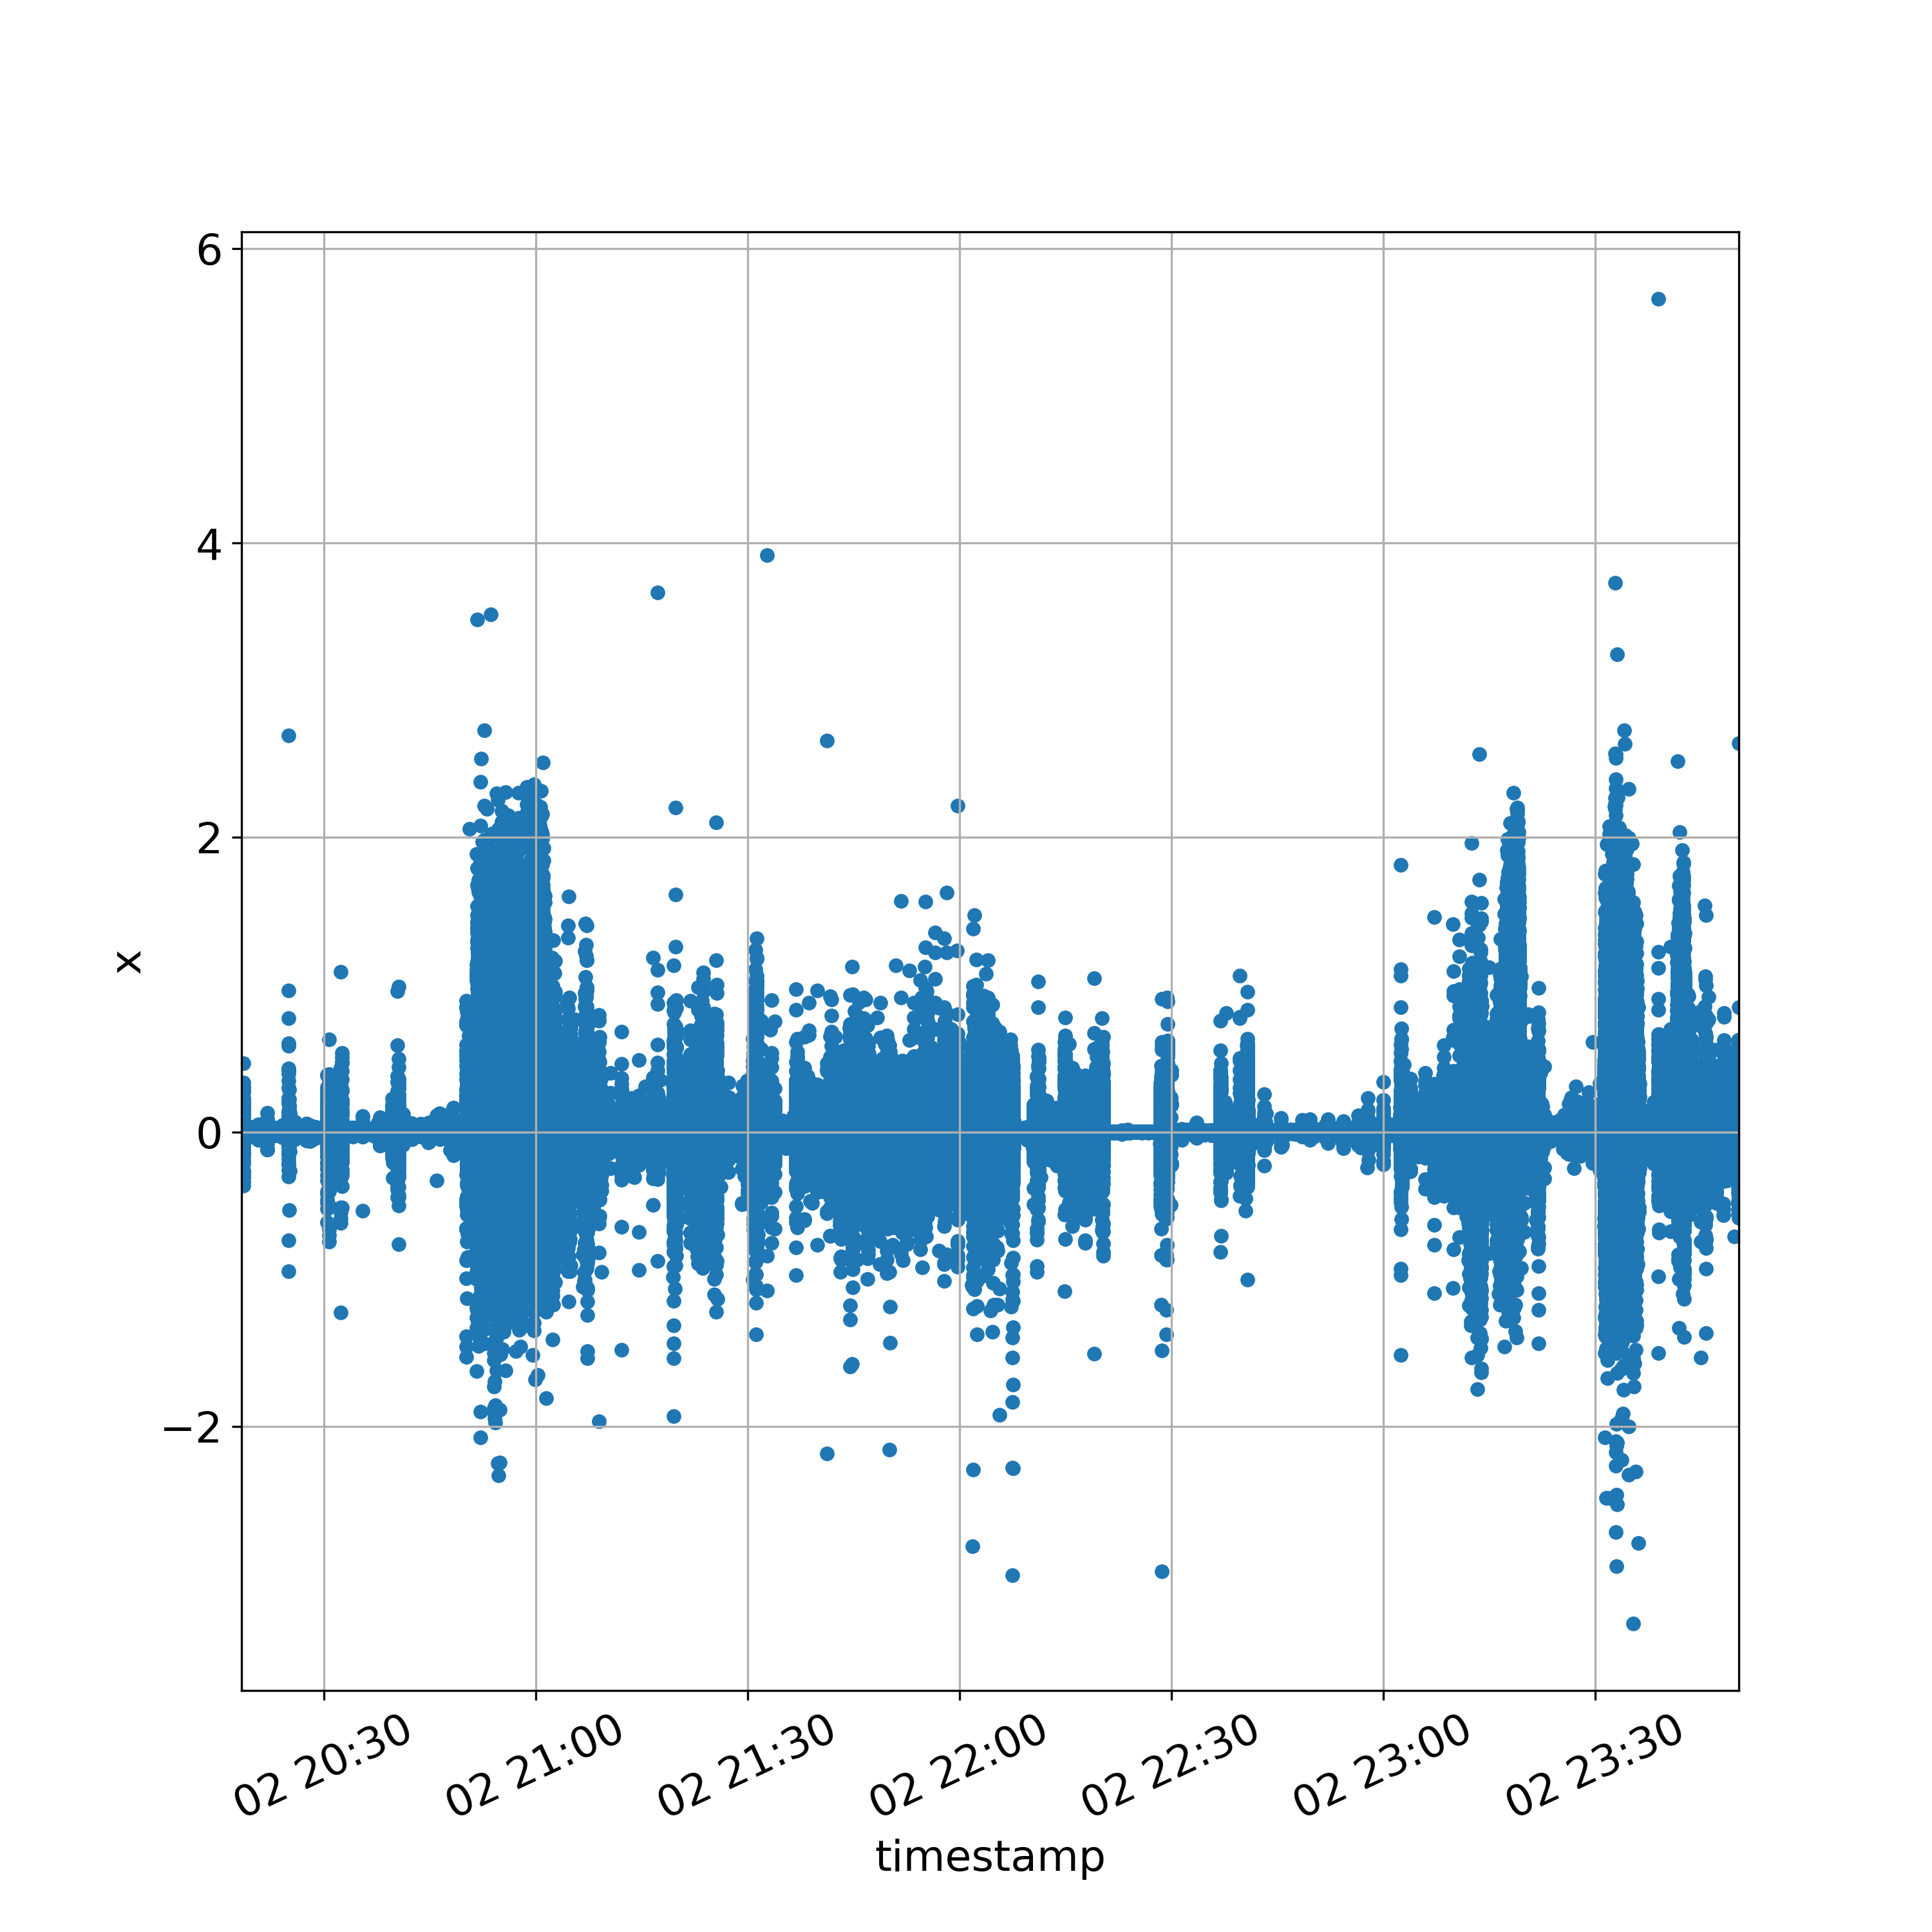
\includegraphics[width=\textwidth]{DC6359_full_x}
		\caption{Accelerometer}
		\label{fig:acc-chunk}		
	\end{subfigure}\hfill%
	\begin{subfigure}[c]{0.49\columnwidth}
		\centering
		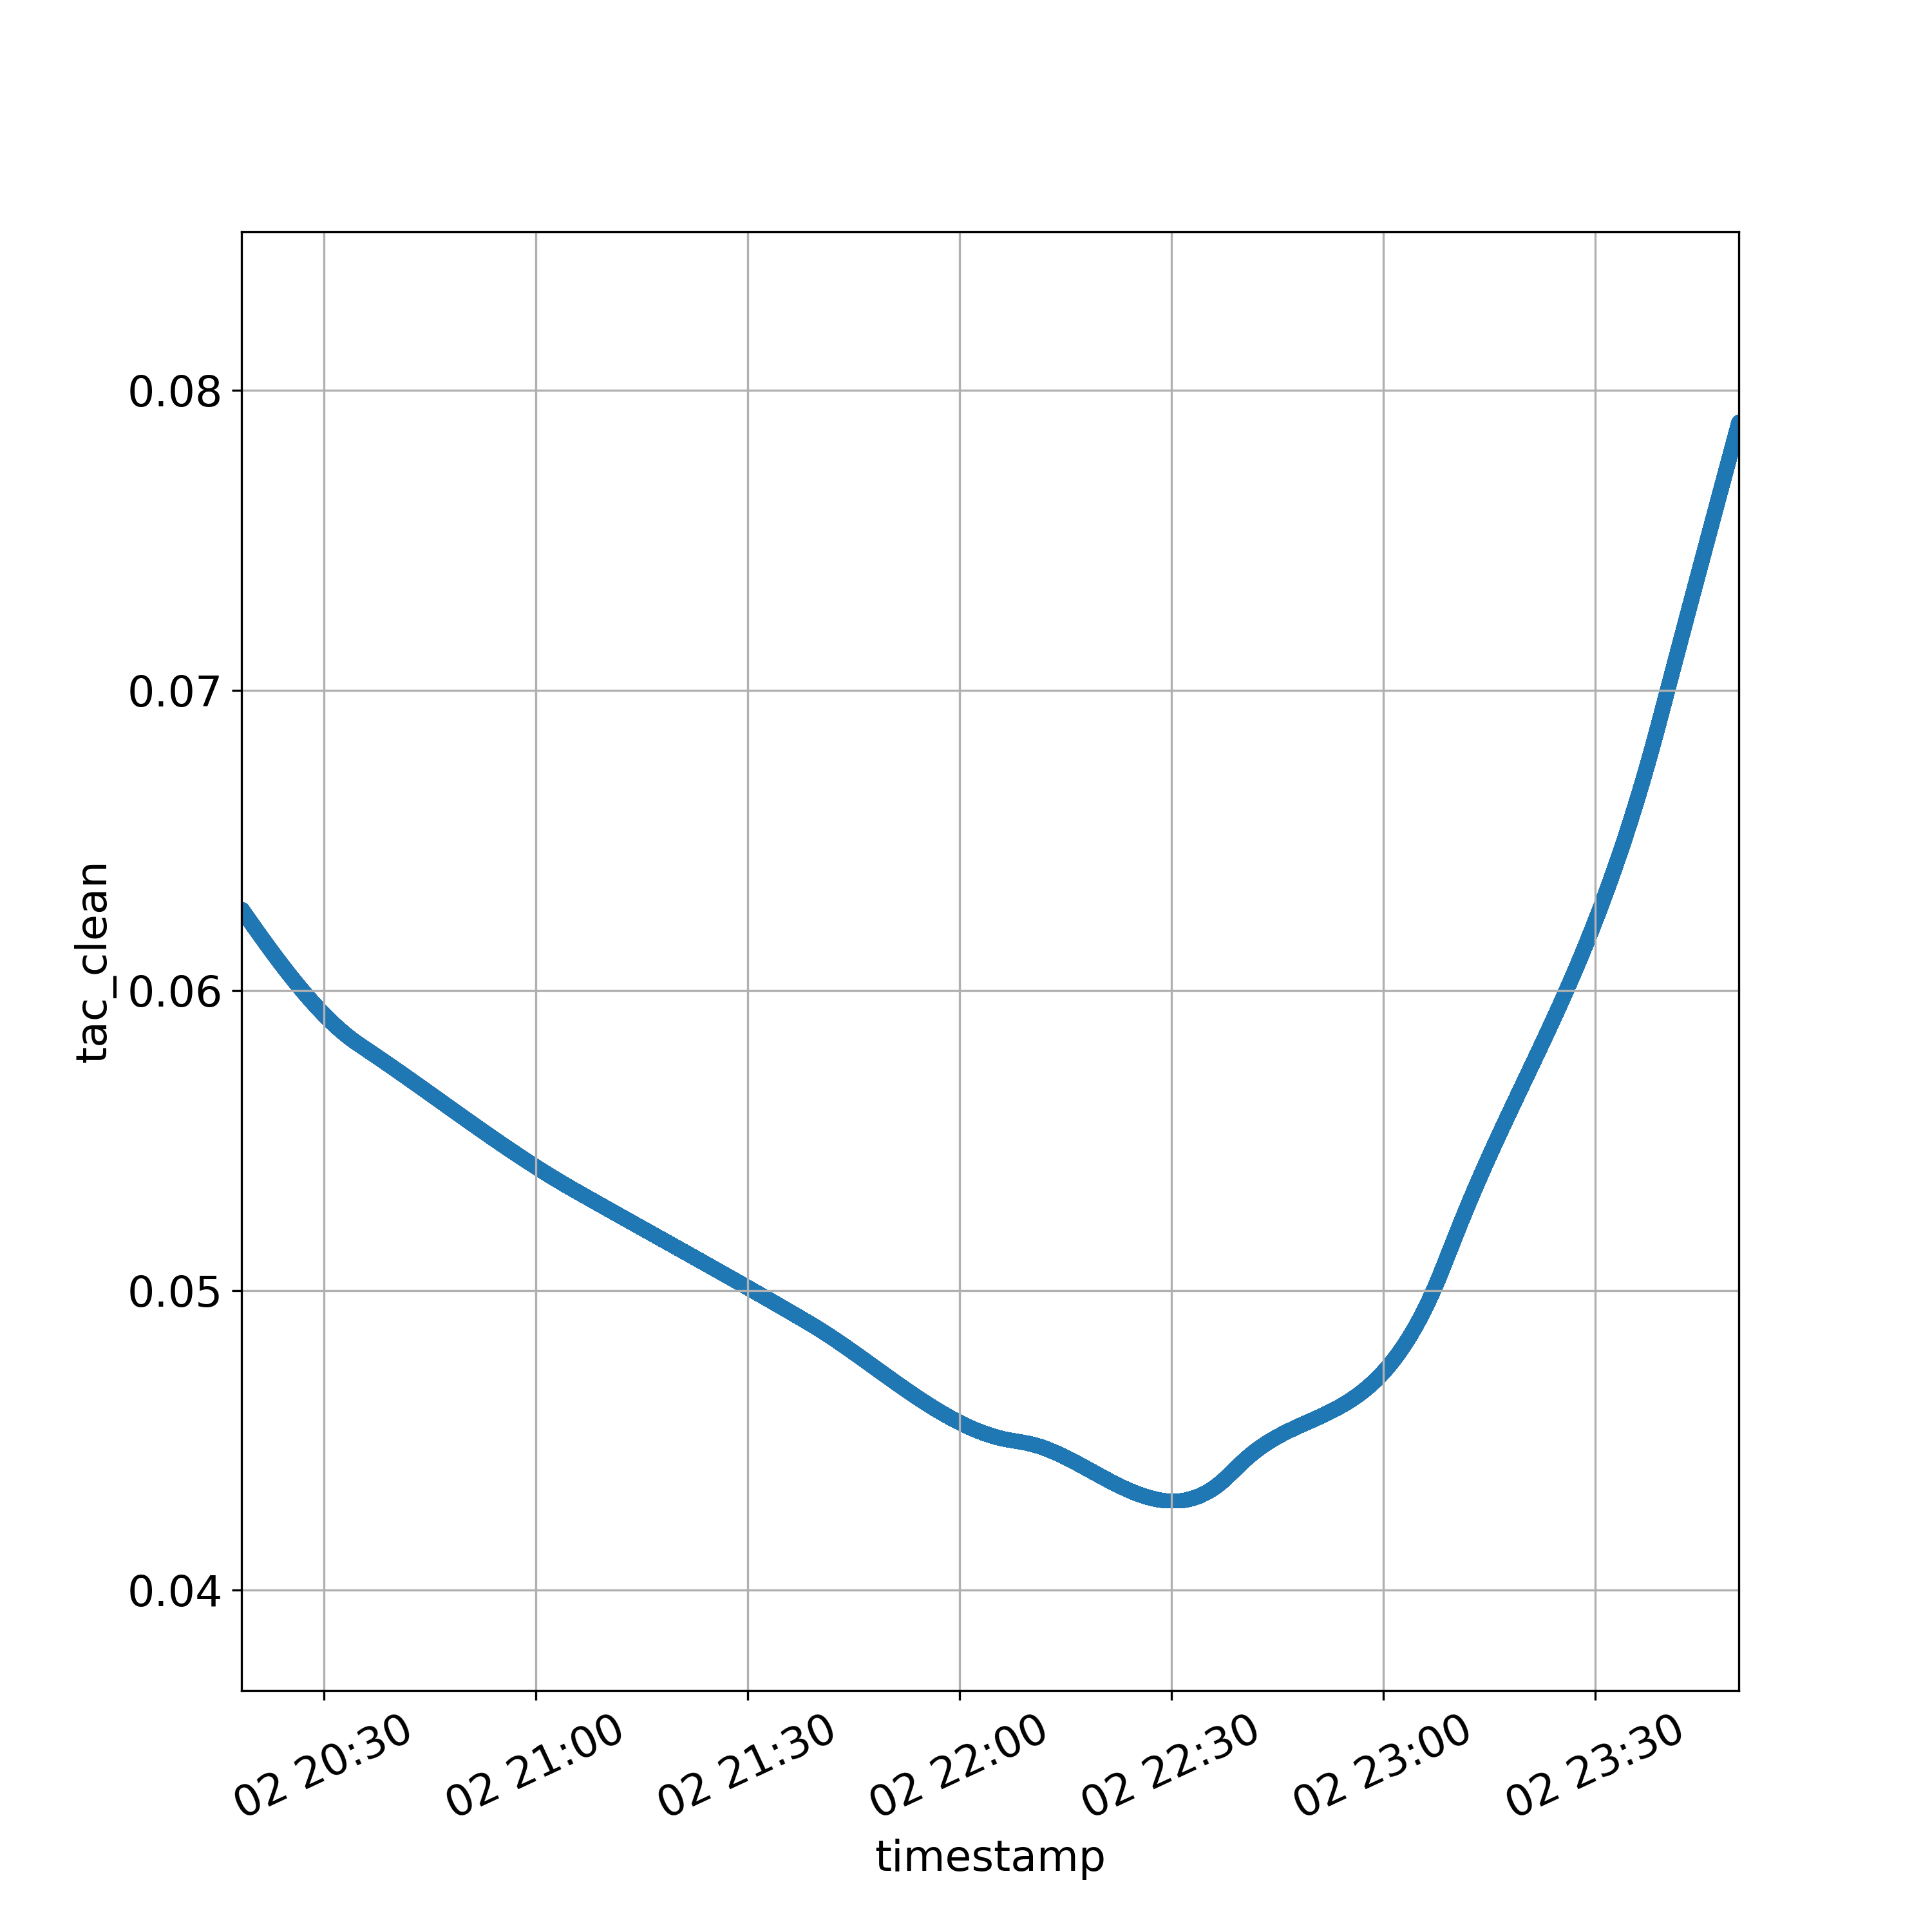
\includegraphics[width=\textwidth]{DC6359_full_clean}
		\caption{TAC}
		\label{fig:tac-chunk}
	\end{subfigure}
	\caption{Chunks of final splitted data for sample \texttt{DC6359}}
\end{figure}

%### Artificial vs Real data...
%### More Detail about the methods

